\chapter{Piattaforma di sviluppo} \label{piattaforma_di_sviluppo}
In questa sezione si descrive come è composta e come è stata assemblata la piattaforma per lo sviluppo e il testing.

\section{Rover AgileX}
Il veicolo selezionato per lo sviluppo della presente tesi è un rover terrestre prodotto da AgileX, modello Hunter. Questo rover è dotato di 3 motori elettrici (2 per la trazione posteriore ed 1 per lo sterzo), di sensori dediti all'analisi del movimento delle ruote e di una board dedicata al controllo dei motori e all'interfacciamento del mezzo con un calcolatore esterno. L'intera scocca è realizzata in alluminio rendendolo molto resistente ma allo stesso tempo non eccessivamente pesante.

\begin{figure}[h]
  \centering
  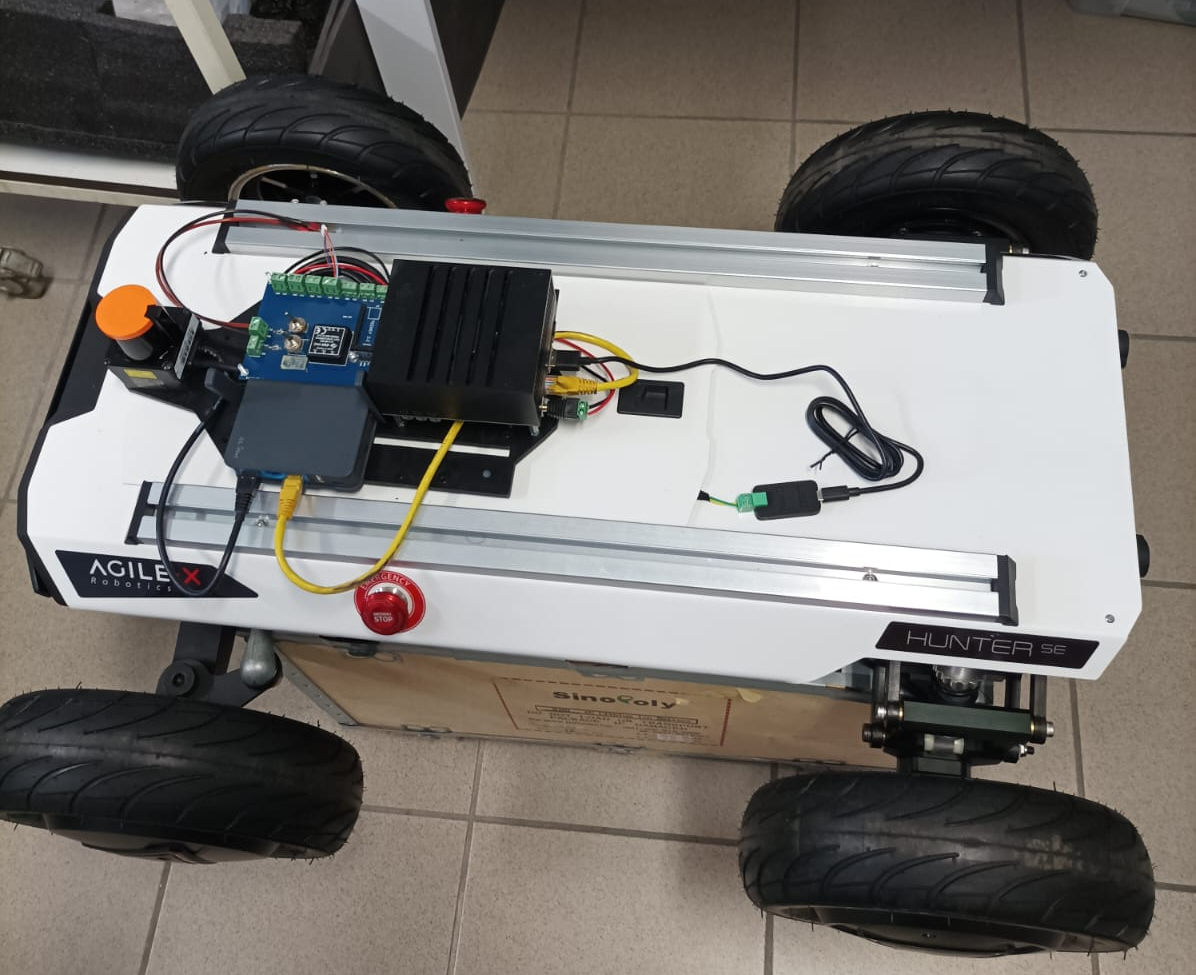
\includegraphics[width=0.8\textwidth]{figures/franco.png}
  \caption{Rover assemblato}
  \label{Rover assemblato}
\end{figure}

\noindent La scheda di controllo del rover è collegata alla porta usb del computer embedded tramite un'apposita periferica e consente una comunicazione efficiente e affidabile. Il modello Hunter è stato scelto per le sue avanzate caratteristiche tecniche e per la sua versatilità, che lo rendono particolarmente adatto alle esigenze del progetto.

\noindent Oltre a fornire un'interfaccia per il controllo diretto, il veicolo è in grado di raccogliere e trasmettere una serie di dati diagnostici e operativi fondamentali per il monitoraggio e l'analisi delle sue prestazioni. Tra questi dati, un ruolo cruciale è ricoperto dall'odometria. 

\noindent L'odometria è una misura che permettte la stima dello spostamento di un veicolo a partire dallo spostamento delle ruote, ed è essenziale per la navigazione e la stima della posizione del rover, poiché permette di determinare il percorso seguito dal veicolo e la distanza percorsa. Questi dati, insieme ad altre informazioni sullo stato del veicolo, contribuiscono a garantire un controllo preciso e ad alimentare i sistemi di guida autonoma e remota previsti dal progetto.

\subsection{Protocollo CAN}
La scheda di controllo del rover è basata sul protocollo Controller Area Network (CAN), un protocollo seriale molto versatile sviluppato dall'azienda Bosh nel 1993 e molto utilizzato in ambito automotive e automazione industriale. Questa interfaccia seriale è accessibile tramite 2 segnali denominati CAN-HIGH e CAN-LOW, collegati ad una periferica USB interfacciata al computer di bordo.

\noindent Il protocollo CAN è utilizzato in quanto è un protocollo molto resistente alle interferenze (grazie a una tecnica di bit dominante e recessivo), veloce e per niente costoso.  

\section{GPGPU}
Un elemento cruciale per la realizzazione di questa tesi è stato l'identificazione e la selezione di un calcolatore embedded che possa comunicare con i sensori e il rover e che possa gestire il carico di tutti gli algoritmi e i processi necessari per la guida autonoma.

\noindent La scelta è ricaduta su una scheda di casa Nvidia, modello AGX Jetson Xavier, una  General Purpose Graphic Processing Unit (GPGPU). Questa scelta è motivata dall'elevata capacità di elaborazione parallela che solo una GPGPU può fornire, capacità che risulta particolarmente vantaggiosa per l'esecuzione di complessi algoritmi di percezione, pianificazione e controllo, da svolgere in tempo reale. La GPGPU selezionata opera con il sistema operativo Ubuntu 20.04 Focal Fossa, noto per la sua stabilità e compatibilità con l'hardware scelto.

\begin{figure}[h]
  \centering
  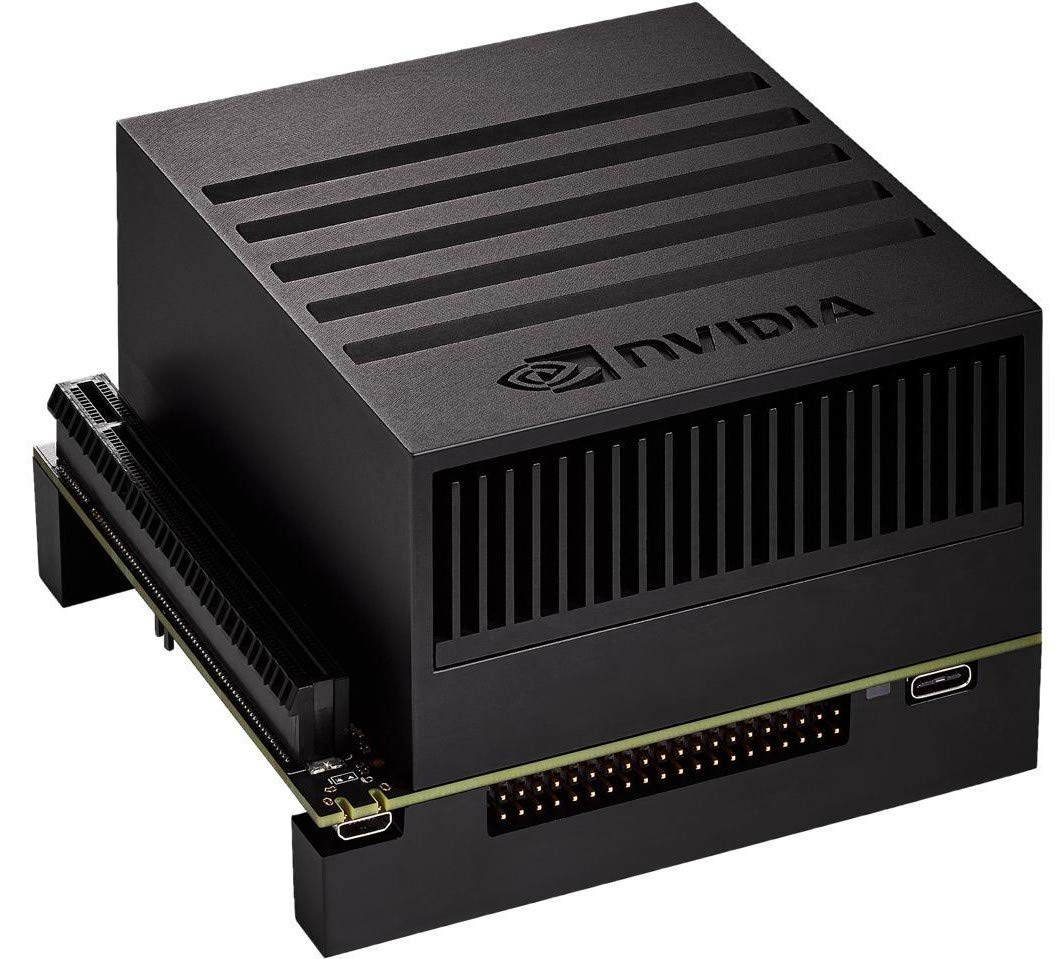
\includegraphics[width=0.65\textwidth]{figures/xavier.jpg}
  \caption{Nvidia AGX Jetson Xavier}
  \label{Nvidia AGX Jetson Xavier}
\end{figure}

\noindent Di seguito una tabella riassuntiva delle principali caratteristiche della GPGPU Utilizzata:

\begin{center}
  \begin{table}[h]
  \centering
    \begin{tabular}{|c|c|}
      \hline 
      GPU& GPU con architettura NVIDIA Volta a 512 core con 64 Tensor Core \\
      \hline 
      CPU& CPU NVIDIA Carmel Arm® v8.2 8-core 64-bit 8 MB L2 + 4 MB L3 \\
      \hline 
      Memoria& LPDDR4x 32 GB 256-bit 136,5 GB/s \\
      \hline
      Storage& eMMC 5.1 32 GB espandibile con scheda di memoria e/o SSD NVMe \\ 
      \hline
      Alimentazione& 10 W - 30 W \\
      \hline
    \end{tabular}
    \caption{Specifiche tecniche della GPGPU Nvidia AGX Jetson Xavier\cite{jetson_xavier}}
  \end{table}
\end{center}

\section{Lidar}
Per permettere al sistema di orientarsi e navigare correttamente è necessario l'utilizzo di un sensore che permetta al veicolo di percepire l'ambiente circostante. La scelta è ricaduta su un sensore Light Detection and Ranging (LiDaR) 2D di marca Hokuio. Questo dispositivo sfrutta la tecnologia laser per determinare la distanza di vari punti nell'ambiente circostante, calcolando il tempo di ritorno dei raggi laser emessi. Il Lidar fornisce una mappa dettagliata della topografia dell'ambiente, consentendo al sistema di percezione di creare rappresentazioni, tridimensionali o bidimensionali, dello stesso e fondamentali per il riconoscimento degli ostacoli, la navigazione, la pianificazione del percorso del veicolo e la mappatura dell'ambiente circostante.

\noindent La combinazione di una GPGPU performante e un sensore Lidar avanzato rappresenta una solida base tecnologica per lo sviluppo di un sistema di guida autonoma e remota altamente efficiente.

\noindent Il sensore Lidar genera una nuvola di punti dell'ambiente circostante attraverso l'emissione di impulsi laser in un cono di 270 gradi. Ciascun punto della nuvola corrisponde alla distanza misurata tra il sensore e un elemento dell'ambiente. La distanza è determinata con accuratezza cronometrando il tempo impiegato dall'impulso laser a percorrere il tragitto andata e ritorno.

Figura \ref{Sensore Lidar} riporta un'immagine del sensore scelto.

\begin{figure}[h]
  \centering
  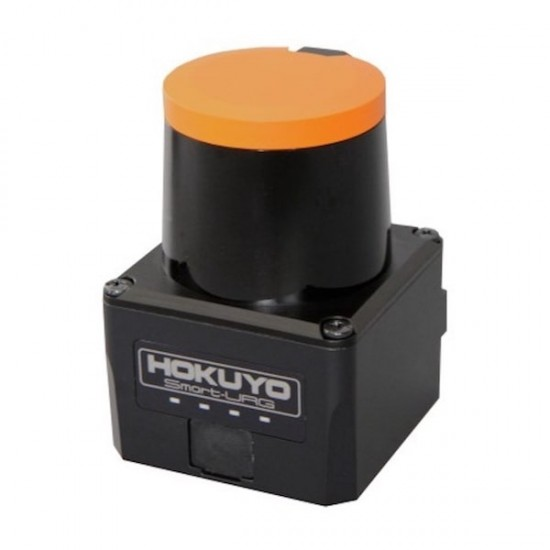
\includegraphics[width=0.65\textwidth]{figures/sensore_hokuio.jpg}
  \caption{Sensore Lidar}
  \label{Sensore Lidar}
\end{figure}

%\newpage
\section{Router}
In considerazione delle elevate esigenze di comunicazione proprie di un veicolo connesso, si è optato per l'integrazione a bordo di un router di rete. Tale dispositivo ha la duplice funzione di instaurare una connessione stabile e ad alta banda passante con l'infrastruttura di rete esterna, garantendo così la trasmissione fluida dei dati, e di fungere da nodo centrale per la comunicazione interna al veicolo. In particolare, il router è preposto a interconnettere il calcolatore di bordo, deputato all'elaborazione dei dati provenienti dai vari sensori, con il sensore Lidar, il quale, mediante interfaccia Ethernet, trasmette ingenti volumi di dati destinati al calcolatore. Il router scelto per il progetto è il modello GL-AR750S di marca gl.inet. Alimentato tramite porta USB direttamente sul rover, questo ruter è noto per le sue piccole dimensioni e il suo basso consumo energetico

\begin{figure}[h]
  \centering
  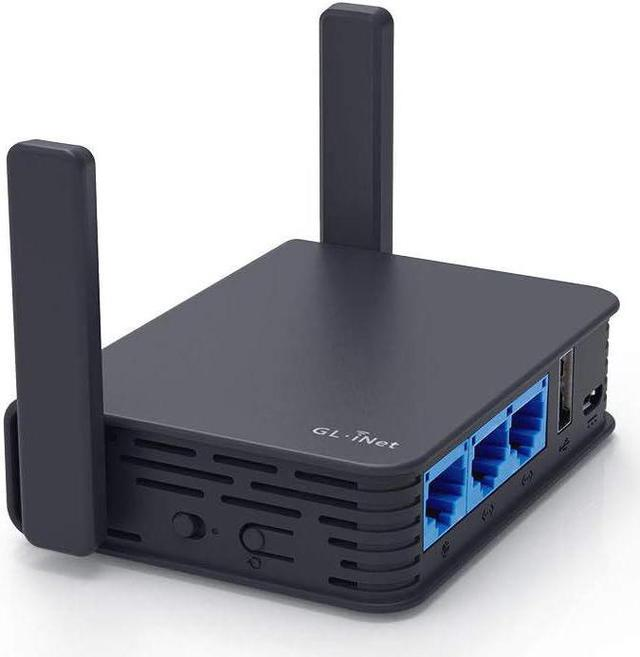
\includegraphics[width=0.65\textwidth]{figures/router.jpg}
  \caption{Router scelto per la piattaforma di sviluppo}
  \label{router}
\end{figure}
